
\begin{figure}
    \centering
    \begin{subfigure}[b]{\textwidth}
        \centering
        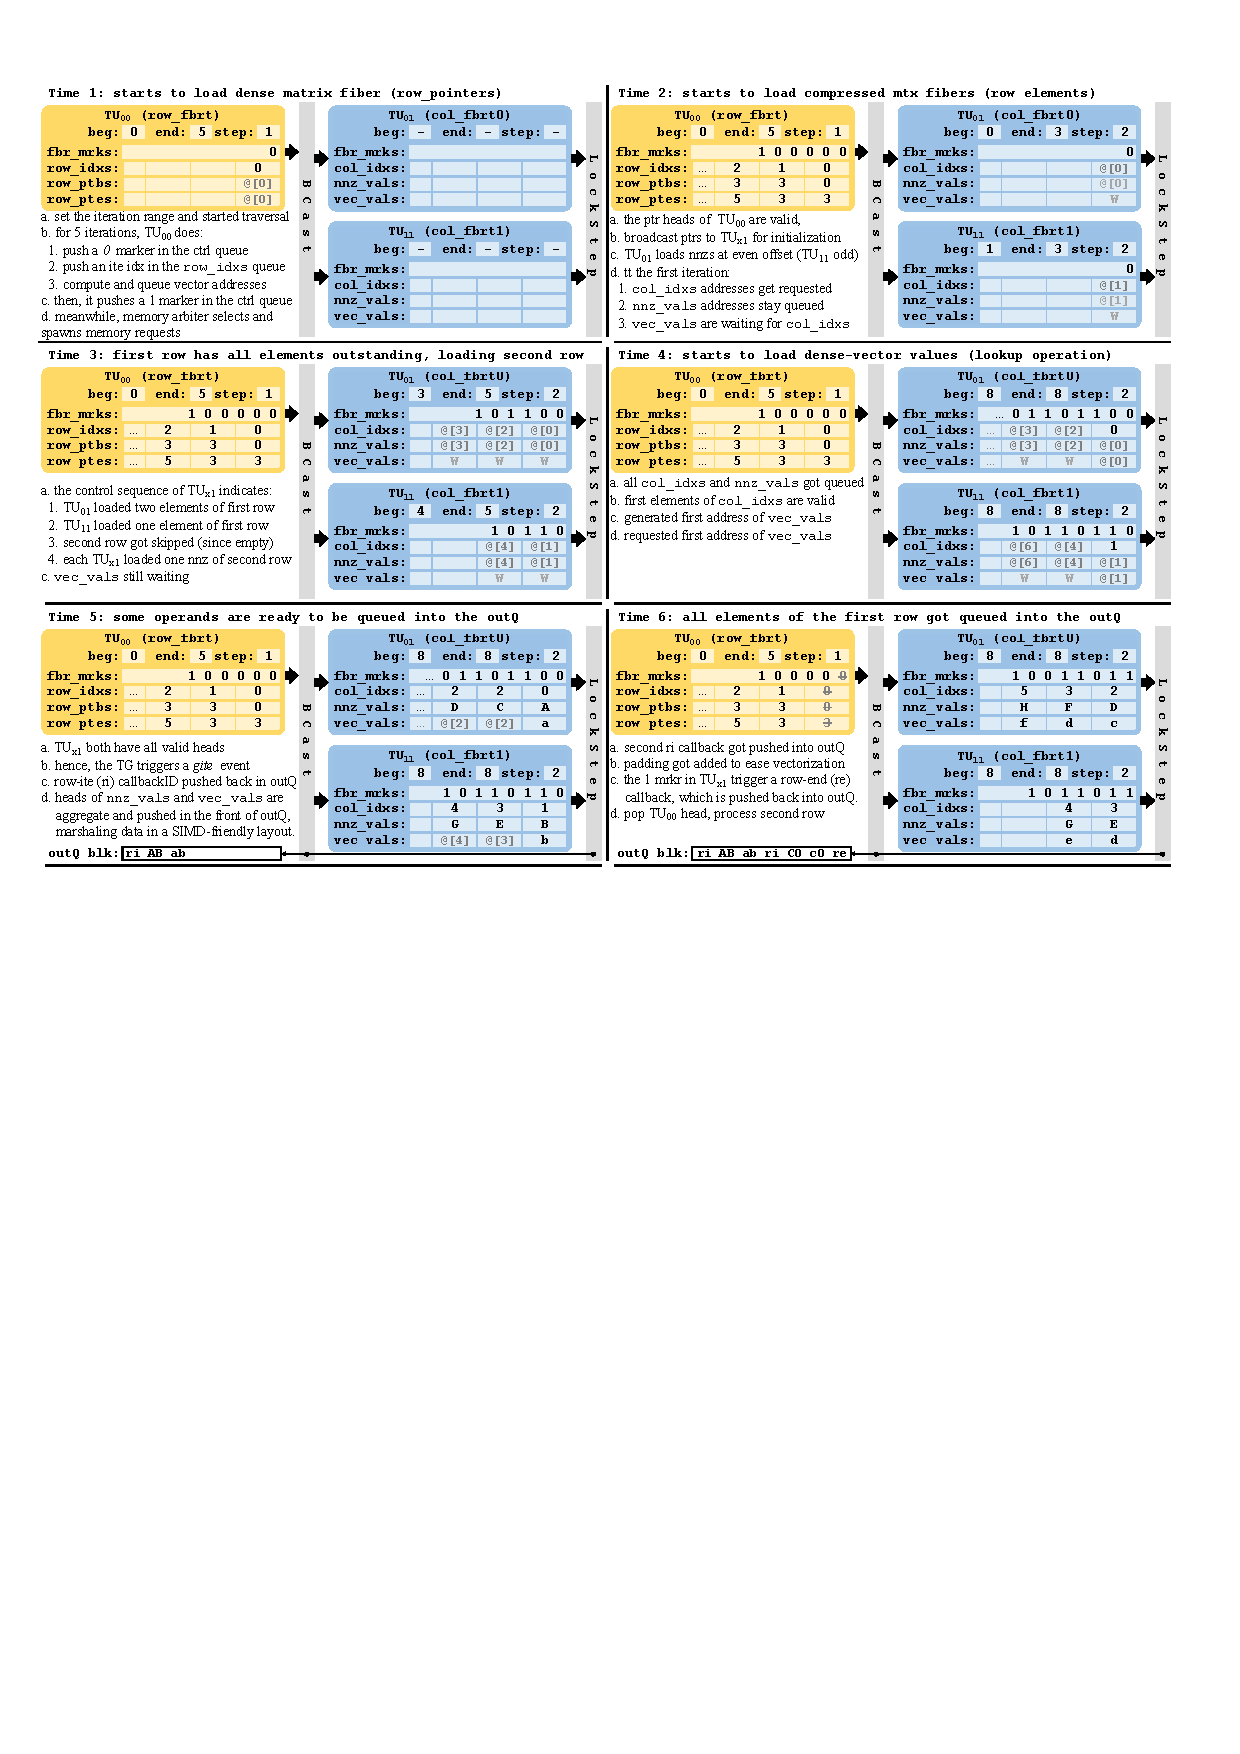
\includegraphics[width=\textwidth,trim=0 260 275 10,clip]{img_spmv_sbs_example.pdf}
        \vspace{-0.5cm}
        \caption{T1: starts to load dense matrix fiber (row\_pointers)}
        \label{fig:sbs-example-t1}
    \end{subfigure}
    \centering
    \begin{subfigure}[b]{\textwidth}
        \centering
        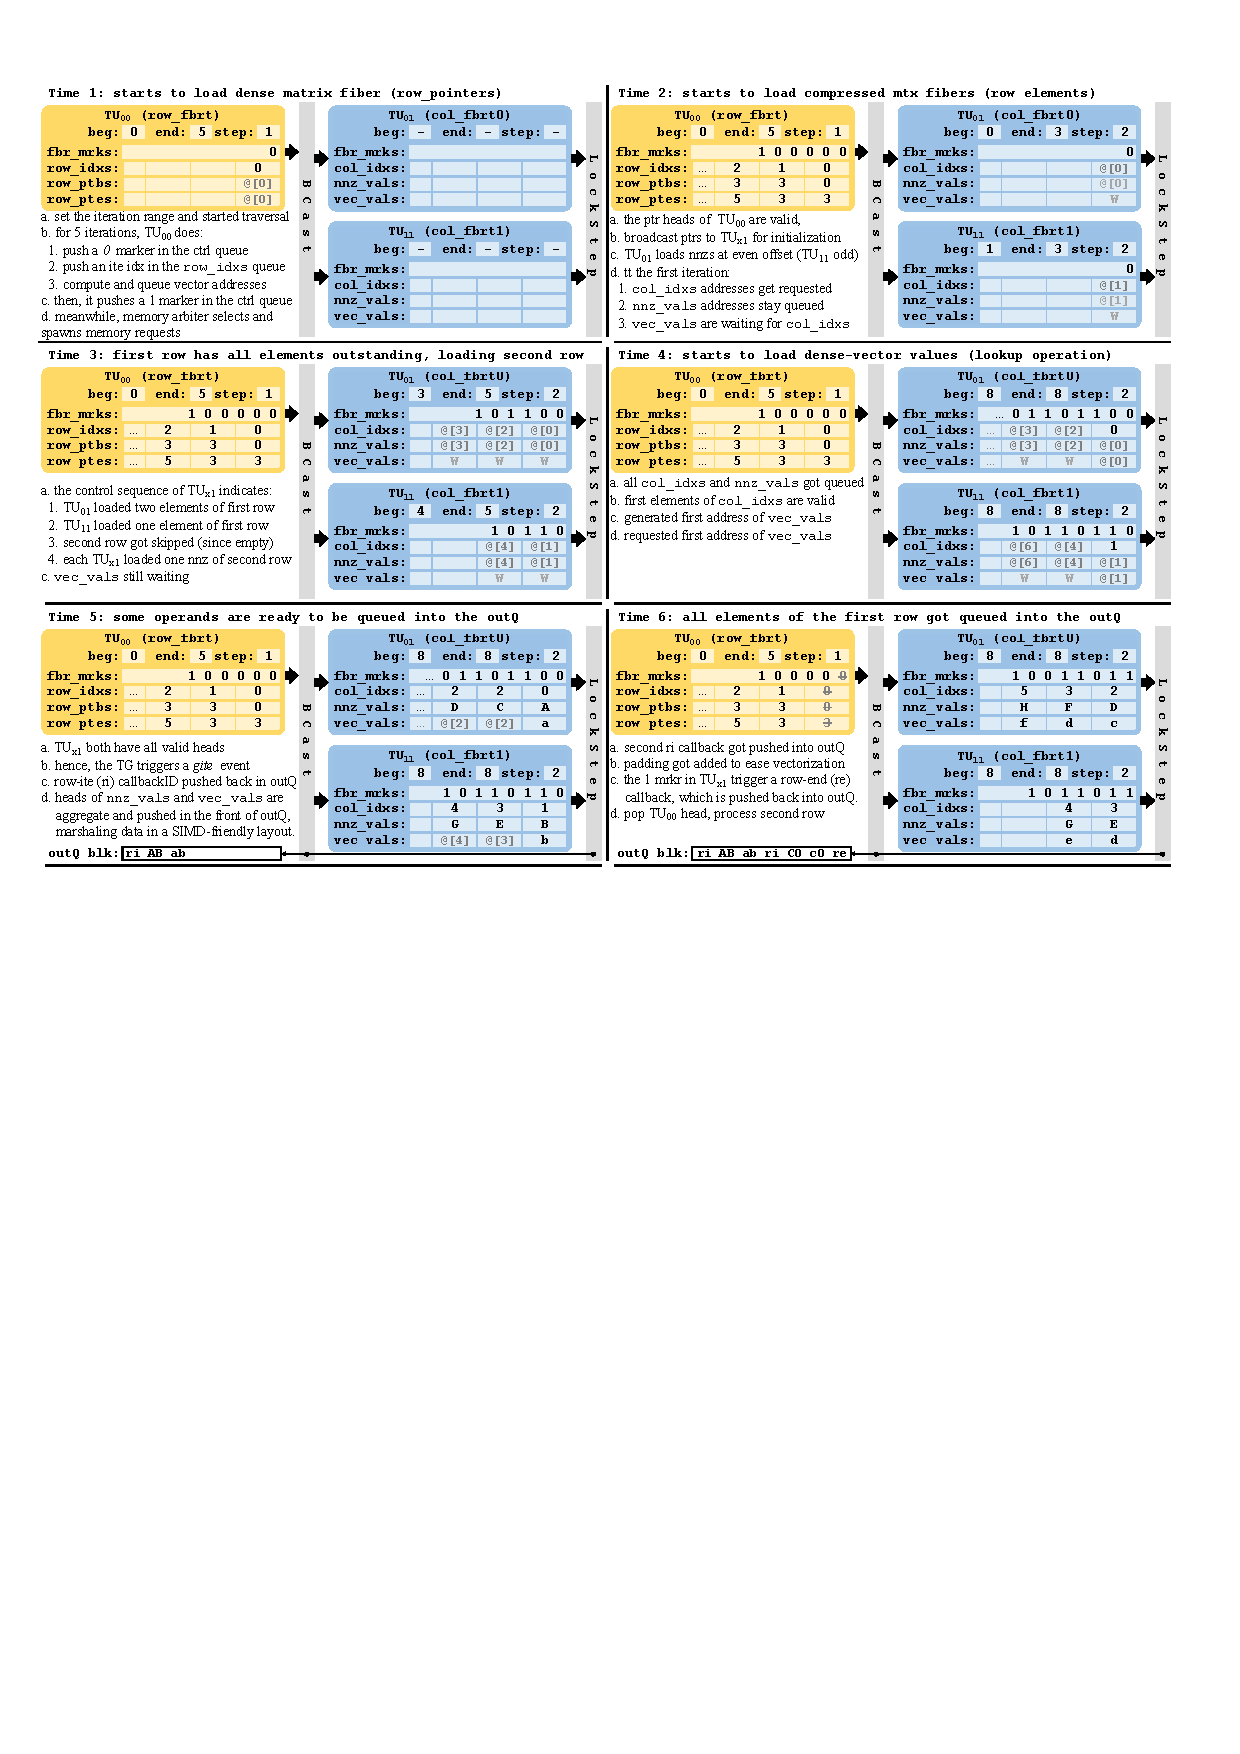
\includegraphics[width=\textwidth,trim=275 260 2 10,clip]{img_spmv_sbs_example.pdf}
        \vspace{-0.5cm}
        \caption{T2: starts to load compressed mtx fibers (row elements)}
        \label{fig:sbs-example-t2}
    \end{subfigure}
    \centering
    \begin{subfigure}[b]{\textwidth}
        \centering
        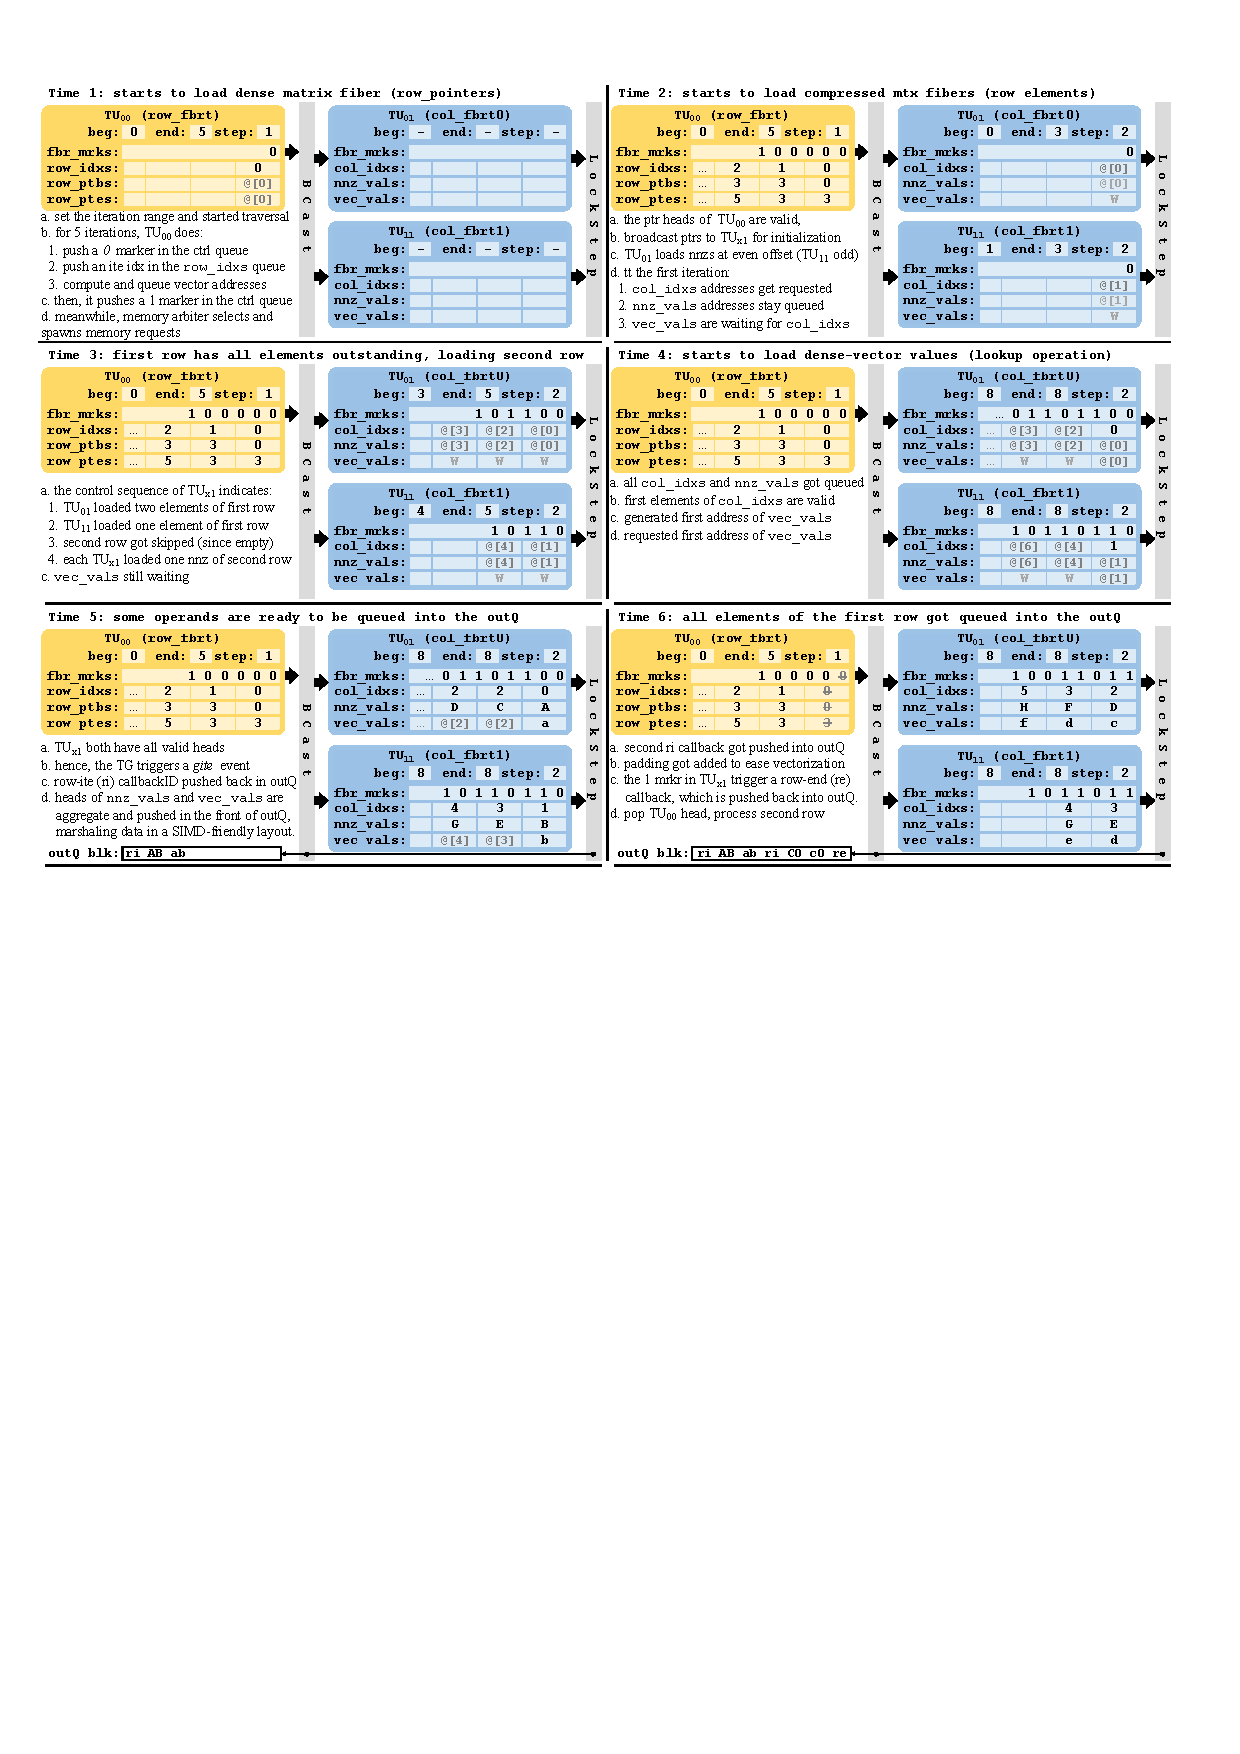
\includegraphics[width=\textwidth,trim=0 130 275 134,clip]{img_spmv_sbs_example.pdf}
        \vspace{-0.5cm}
        \caption{T3: first row has all elements outstanding, loading second row}
        \label{fig:sbs-example-t3}
    \end{subfigure}
    %\vspace{-1em}
  \caption[Step-by-step TMU execution for SpMV, part 1.]{First part of the step-by-step TMU execution of SpMV with inner-loop vectorization (P1 in \Cref{tab:tensor-mapping}) over the CSR matrix in \Cref{fig:sparse-formats}. T1 loads the row-pointer fiber, T2 starts the compressed row traversal, and T3 has issued all requests for the first row while beginning the next row. This shows how the TMU exposes memory-level parallelism before operands are ready for computation.}
  \label{fig:spmv-step-1}
\end{figure}

\begin{figure}
    \centering
    \begin{subfigure}[b]{\textwidth}
        \centering
        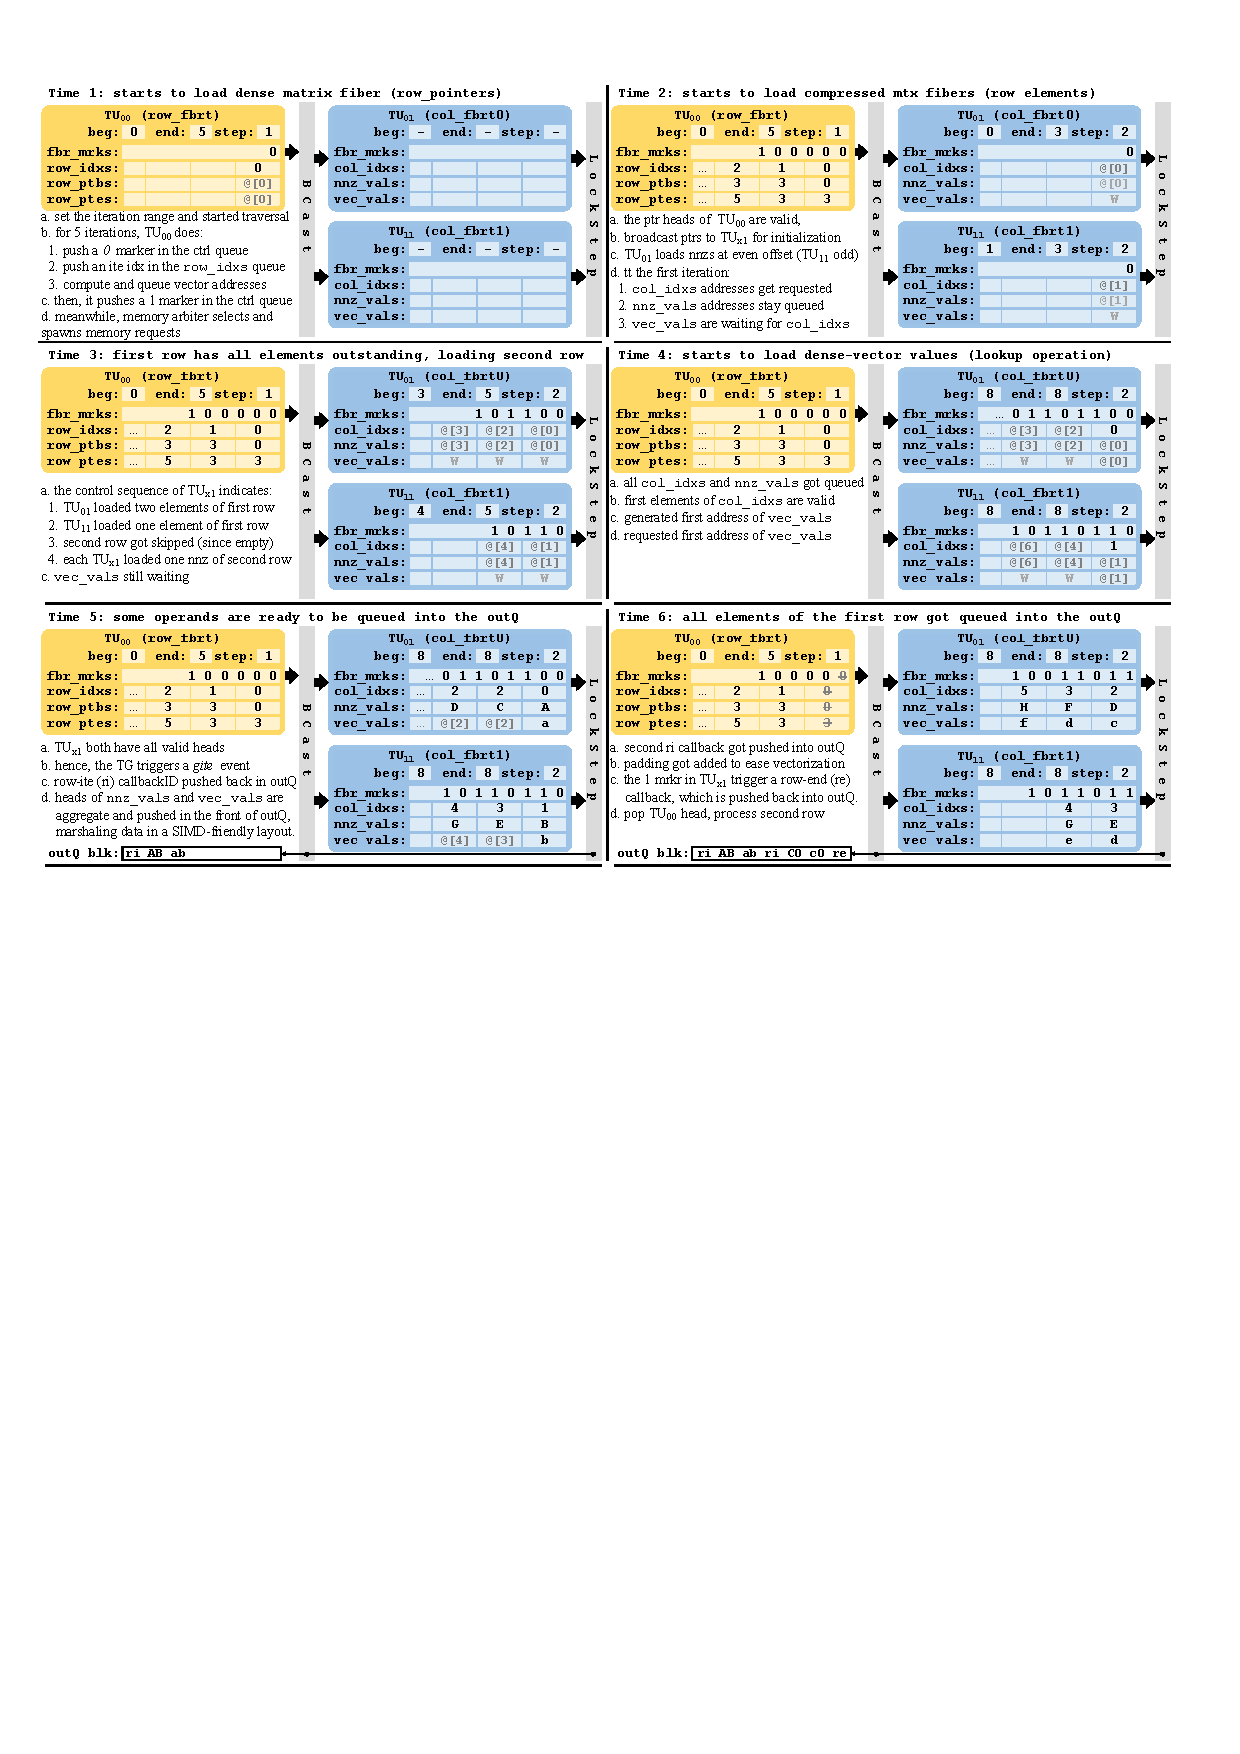
\includegraphics[width=\textwidth,trim=275 130 2 134,clip]{img_spmv_sbs_example.pdf}
        \vspace{-0.5cm}
        \caption{T4: starts to load dense-vector values (lookup operation)}
        \label{fig:sbs-example-t4}
    \end{subfigure}
    \centering
    \begin{subfigure}[b]{\textwidth}
        \centering
        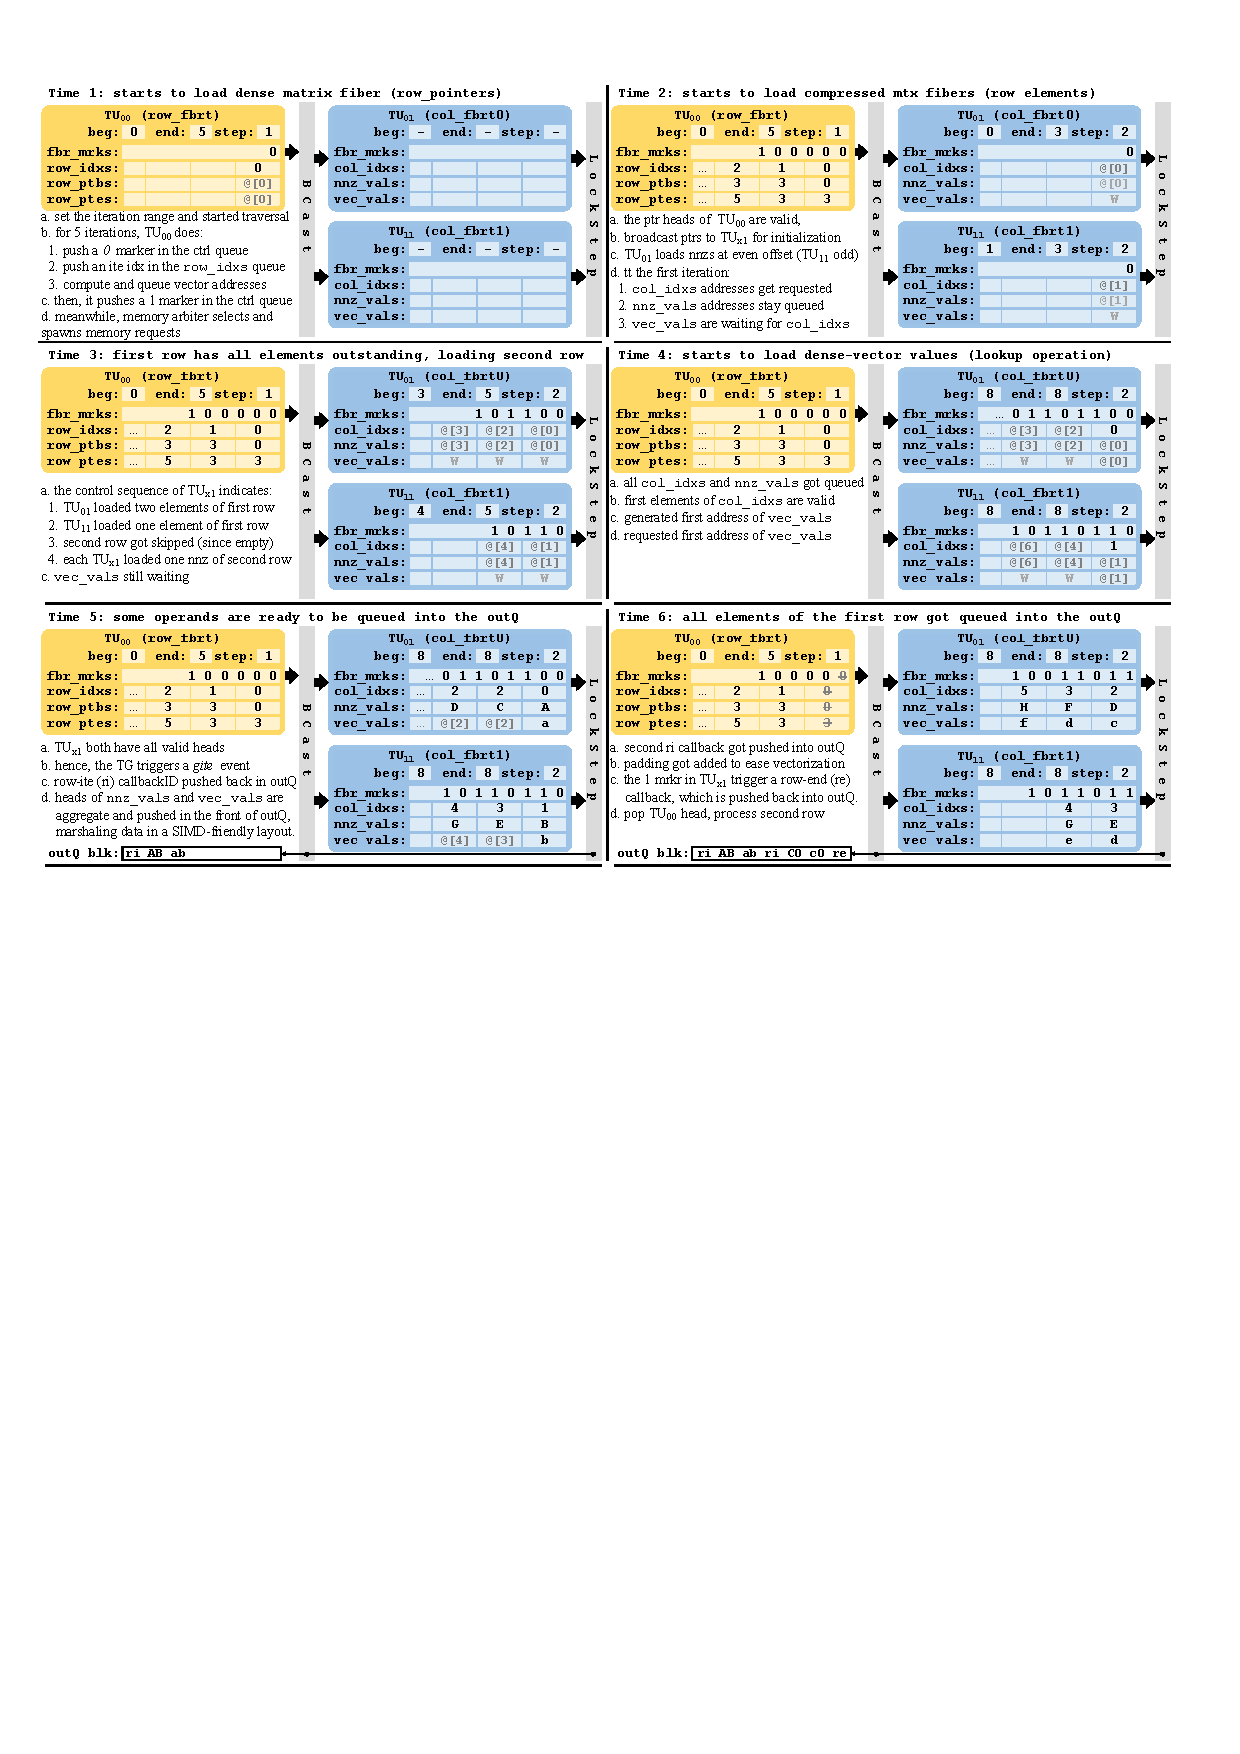
\includegraphics[width=\textwidth,trim=0 4 275 260,clip]{img_spmv_sbs_example.pdf}
        \vspace{-0.5cm}
        \caption{T5: some operands are ready to be queued into the outQ}
        \label{fig:sbs-example-t5}
    \end{subfigure}
    \centering
    \begin{subfigure}[b]{\textwidth}
        \centering
        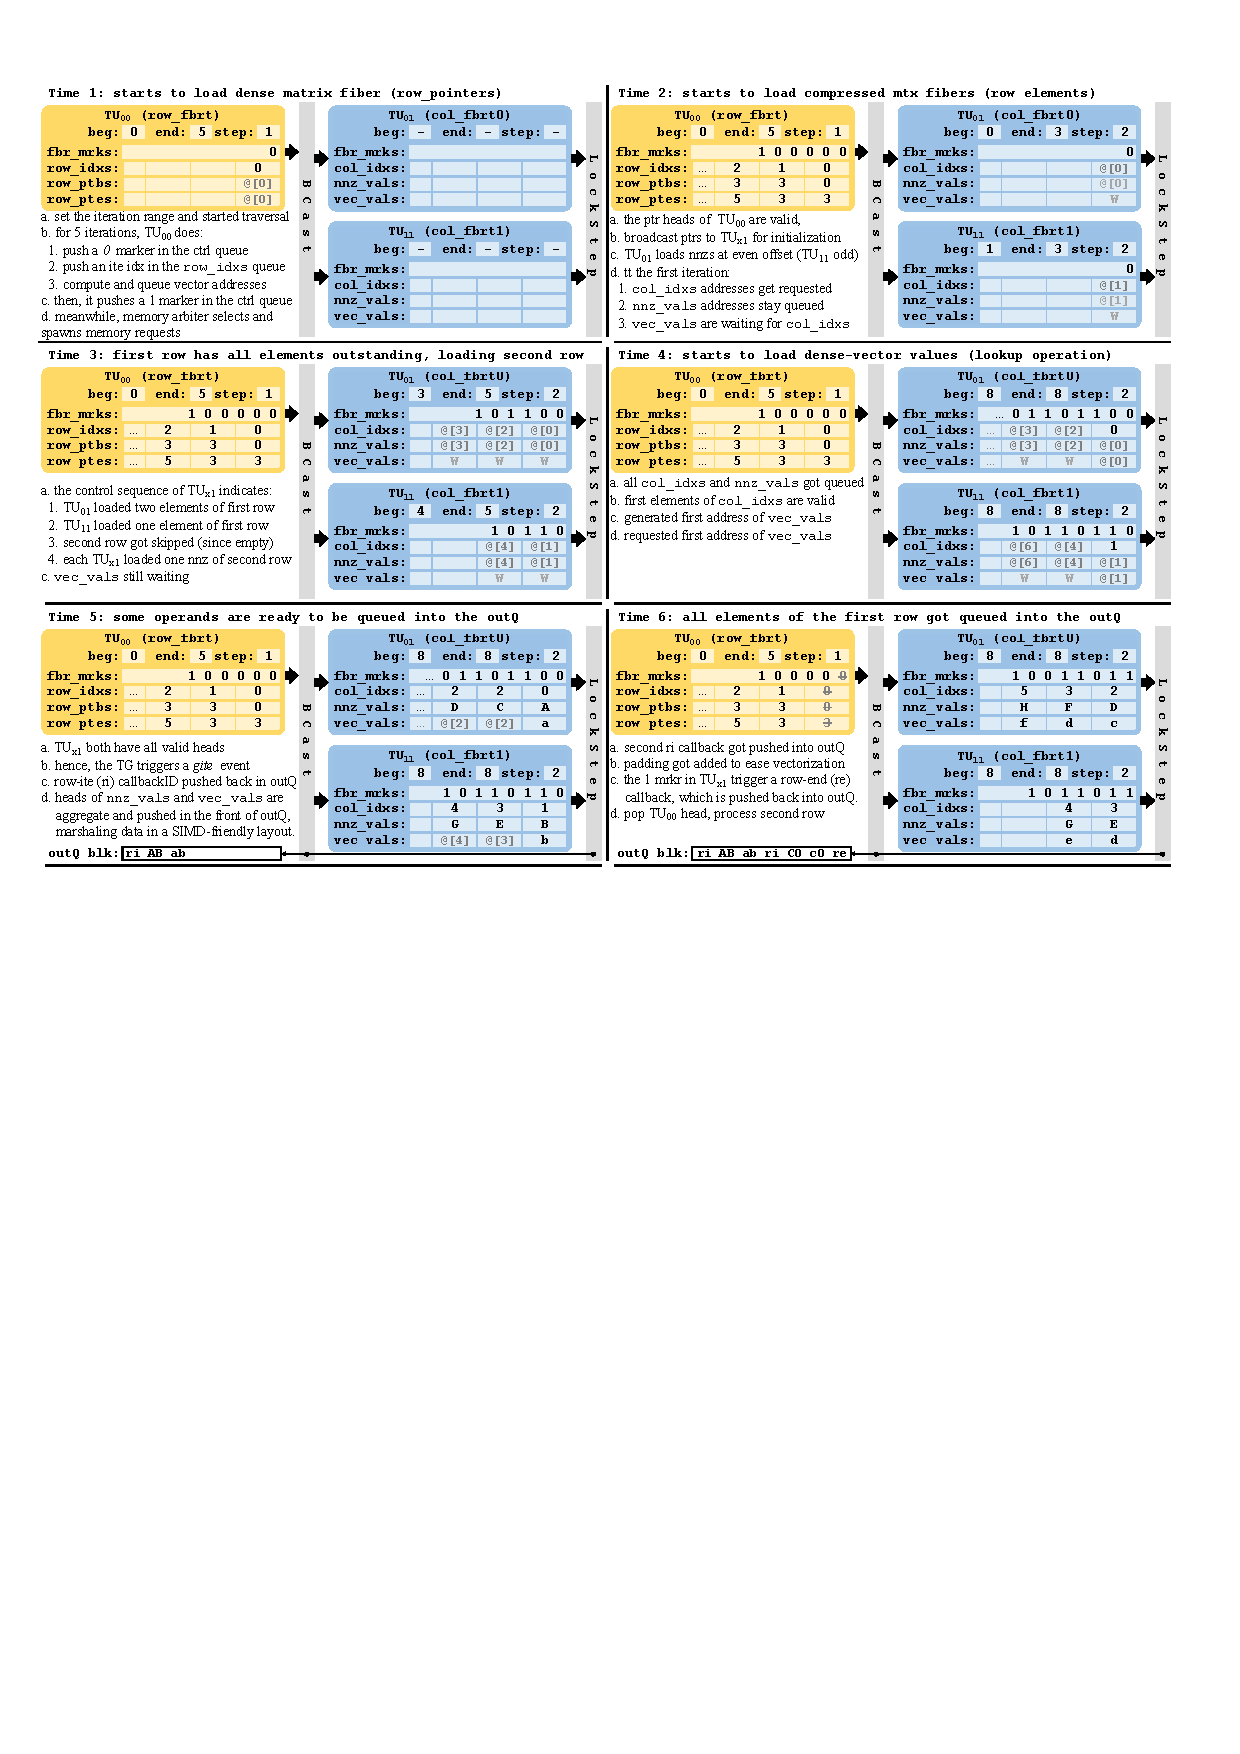
\includegraphics[width=\textwidth,trim=275 4 2 260,clip]{img_spmv_sbs_example.pdf}
        \vspace{-0.5cm}
        \caption{T6: all elements of the first row got queued into the outQ}
        \label{fig:sbs-example-t6}
    \end{subfigure}
    %\vspace{-1em}
  \caption[Step-by-step TMU execution for SpMV, part 2.]{Second part of the step-by-step TMU execution of SpMV with inner-loop vectorization (P1 in \Cref{tab:tensor-mapping}) over the CSR matrix in \Cref{fig:sparse-formats}. T4 issues dense-vector lookups, T5 begins marshaling ready operands into the outQ, and T6 has queued all operands for the first row. This shows how traversal results become ordered callback operands for the core.}
  \label{fig:spmv-step-2}
\end{figure}

%\begin{figure}
%\centering
%  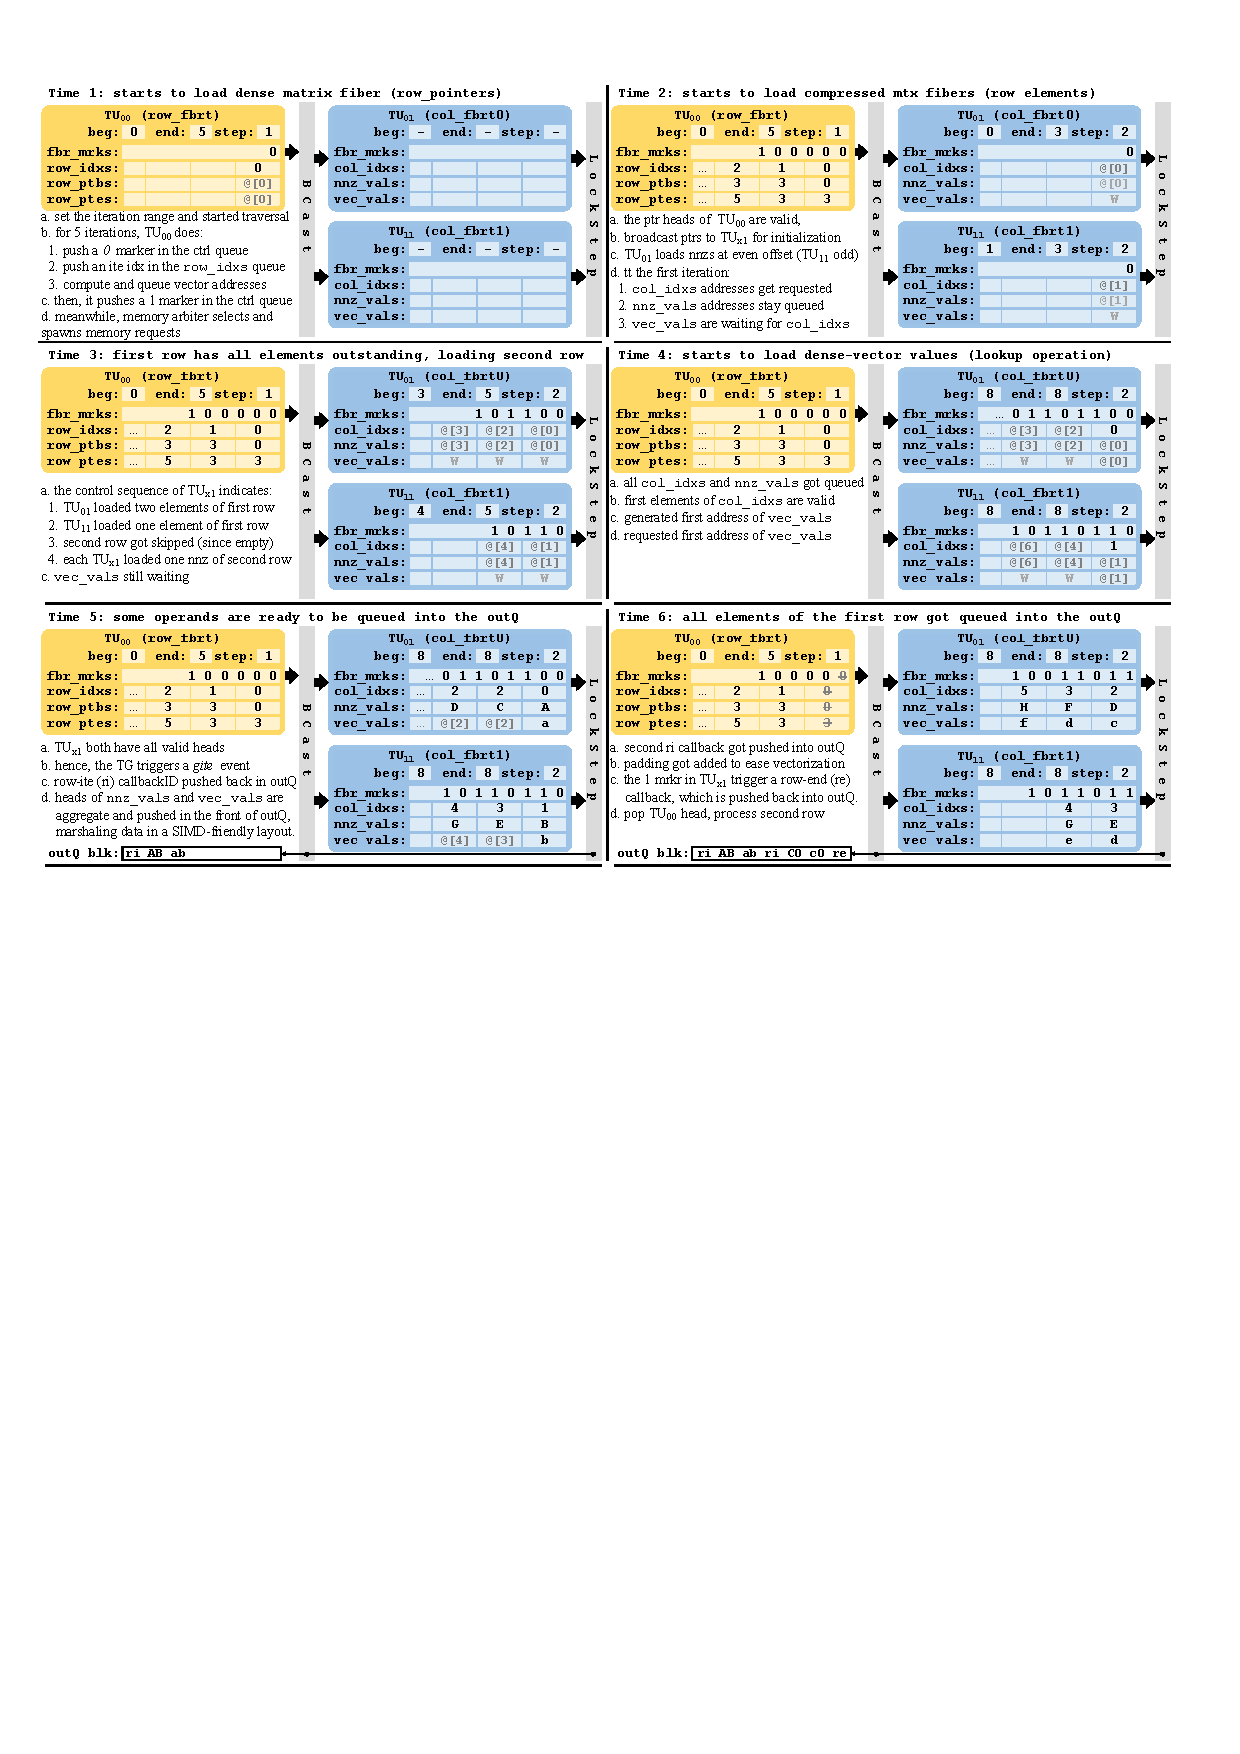
\includegraphics[width=\textwidth]{img_spmv_sbs_example.pdf}
%  \caption{Example performing SpMV with inner-loop vectorization (see \Cref{tab:tmu-data-streams}, P1 version) over the first row of the CSR matrix in %\Cref{fig:sparse-formats}.}
%  \label{fig:spmv_example}
%\end{figure}
